%% ============================================================
%% ICIIT 2027 - ACM sigconf paper
%% Files in the same folder: main.tex, references.bib and five figures
%% (every figure is produced by Notebook A or B and keeps its name from report/;
%%  here they are downsized copies so that Overleaf's free plan compiles in time).
%% ============================================================

\documentclass[sigconf]{acmart}

\usepackage{booktabs}
\usepackage{subcaption}
\microtypesetup{expansion=false} % faster compile on Overleaf free plan

%% --- submission settings: no copyright block, no ACM reference format ---
\settopmatter{printacmref=false}
\setcopyright{none}
\renewcommand\footnotetextcopyrightpermission[1]{}
\pagestyle{plain}

\acmConference[ICIIT 2027]{2027 12th International Conference on Intelligent Information Technology}{March 04--07, 2027}{Ho Chi Minh City, Vietnam}
\acmYear{2027}

\begin{document}

\title[Data Repair Steps in Next-Hour Traffic Forecasting]{What Each Data Repair Step Is Worth in Next-Hour Traffic Forecasting on the Istanbul Open Data and What Happens on Holidays}

\author{Quang Tran}
\affiliation{\institution{FPT University}\city{Ho Chi Minh City}\country{Vietnam}}
\email{tranquangsc0123@gmail.com}

\author{An Truong}
\affiliation{\institution{FPT University}\city{Ho Chi Minh City}\country{Vietnam}}
\email{tnban10a32122@gmail.com}

\author{Loc Truong}
\affiliation{\institution{FPT University}\city{Ho Chi Minh City}\country{Vietnam}}
\email{truongtanloc00@gmail.com}

\author{Thu Le}
\affiliation{\institution{FPT University}\city{Ho Chi Minh City}\country{Vietnam}}
\email{thulvm@fpt.edu.vn}

\begin{abstract}
Papers on short-term traffic forecasting usually report one error number and say little about how much of it comes from data preparation rather than from the model. We measure this on the hourly traffic density open data of Istanbul (36 monthly files, 2022--2024, 58.4 million records), restricted to the 150 busiest road cells. Over eight quarterly test folds with an expanding training window, four models (Ridge, Extra Trees, LightGBM, MLP) forecast the next-hour vehicle count against persistence and three simple baselines, and data repair steps are added one at a time. LightGBM and the MLP reach a mean absolute error (MAE) of about 38 vehicles per cell-hour, 44\% below persistence, but differ by less than the spread between test quarters. The repair steps together lower the mean MAE of the four models from 46.1 to 40.8, and 4.2 of these 5.3 vehicles come from one step: placing the data on a complete hourly grid. After a public holiday the usual ``same hour last week'' feature points at an atypical day, and the error peaks exactly seven days after the holiday starts (66.8 against 38.5 on the holiday itself). Taking the lag from the nearest ordinary week lowers the week-after-holiday MAE from 54.2 to 41.8 while costing 0.2 vehicles on ordinary days. We also document an unexplained level shift in the source data in January 2024.
\end{abstract}

\begin{CCSXML}
<ccs2012>
<concept>
<concept_id>10010147.10010257</concept_id>
<concept_desc>Computing methodologies~Machine learning</concept_desc>
<concept_significance>500</concept_significance>
</concept>
<concept>
<concept_id>10002951.10002952.10003219.10003218</concept_id>
<concept_desc>Information systems~Data cleaning</concept_desc>
<concept_significance>500</concept_significance>
</concept>
<concept>
<concept_id>10010405.10010481.10010485</concept_id>
<concept_desc>Applied computing~Transportation</concept_desc>
<concept_significance>500</concept_significance>
</concept>
</ccs2012>
\end{CCSXML}

\ccsdesc[500]{Computing methodologies~Machine learning}
\ccsdesc[500]{Information systems~Data cleaning}
\ccsdesc[500]{Applied computing~Transportation}

\keywords{traffic forecasting, data repair, holidays, open data, Istanbul, time-series validation}

\maketitle

%% ============================================================
\section{Introduction}
Short-term traffic forecasting is a mature topic \cite{vlahogianni2014,lana2018}, and deep or tree-based models report strong accuracy on public data \cite{lv2015,li2018dcrnn,yu2018stgcn}. Most of these studies start from a table that somebody has already cleaned. Open municipal data rarely look like that: sensors go silent for hours, files contain gaps, and calendar effects such as religious holidays are not part of the records. The accuracy reported after cleaning is then a mixture of the model and of many small data decisions that are not measured.

Two such decisions are easy to miss: when hours are missing, the ``previous row'' of a raw table is not always the previous hour; and a holiday breaks the weekly rhythm, so one week later a model that leans on the same hour last week inherits the holiday. We call this the \emph{holiday echo}.

The Istanbul data have been used for a traffic graph benchmark \cite{olug2024}, for LSTM and XGBoost models tuned by grey wolf optimisation \cite{subasi2025} and for explainable incident-impact prediction \cite{korkmaz2026}. None of them reports how much each preparation step changes the error or scores holidays separately, although data decisions that misalign time are a known source of over-optimistic results \cite{kapoor2023}. We contribute (i) a reproducible pipeline from the 36 raw files to a leakage-free SQL feature table; (ii) a repair ladder (R0--R5) scored on the same cells and hours; (iii) a measurement of the holiday echo and of five weekly lags (L0--L4); and (iv) an account of a level break in the source data. Figure~\ref{fig:pipeline} summarises the study.

\begin{figure*}[t]
  \centering
  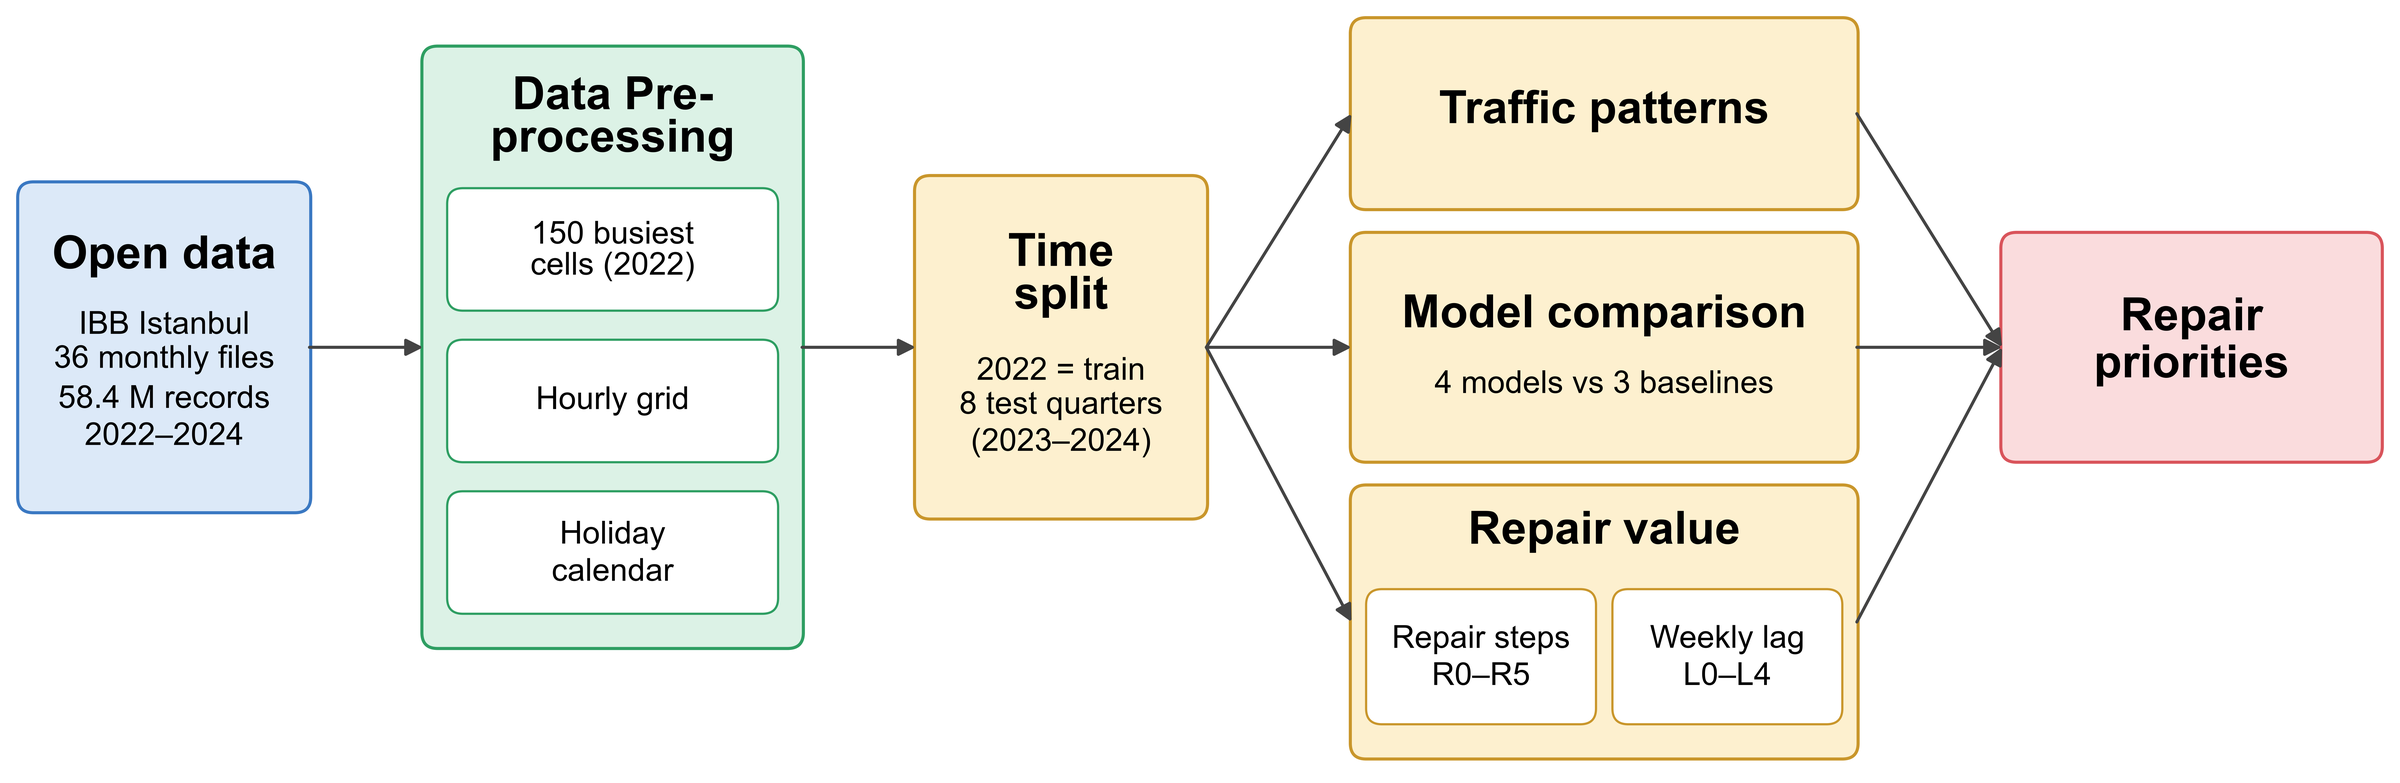
\includegraphics[width=0.9\textwidth]{fig_pipeline.png}
  \caption{Study pipeline. The open data are reduced to the 150 busiest cells of 2022, placed on a complete hourly grid with a holiday calendar, split in time, and used for three analyses that lead to a ranking of repair priorities.}
  \label{fig:pipeline}
\end{figure*}

%% ============================================================
\section{Data}
\subsection{Source and selection of cells}
The IBB portal publishes one CSV file per month with, for every geohash cell and hour, the number of vehicles and their average speed \cite{ibb}. We use all 36 files from January 2022 to December 2024 (58{,}393{,}117 records, no duplicate keys or implausible values).

To avoid looking at the test years, the cells are chosen from 2022 only. Of 2{,}459 cells reporting in 2022, 2{,}385 cover at least half of the hours, and we keep the 150 with the highest mean traffic (245.8--503.5 vehicles per hour). The list is then fixed for 2023 and 2024. The selected cells follow the motorways and the two Bosphorus bridges and split almost evenly between the European (74) and the Asian (76) side (Figure~\ref{fig:map}). They hold 3{,}708{,}004 records, which fill 93.98\% of the complete grid of 3{,}945{,}600 cell-hours.

\begin{figure}[t]
  \centering
  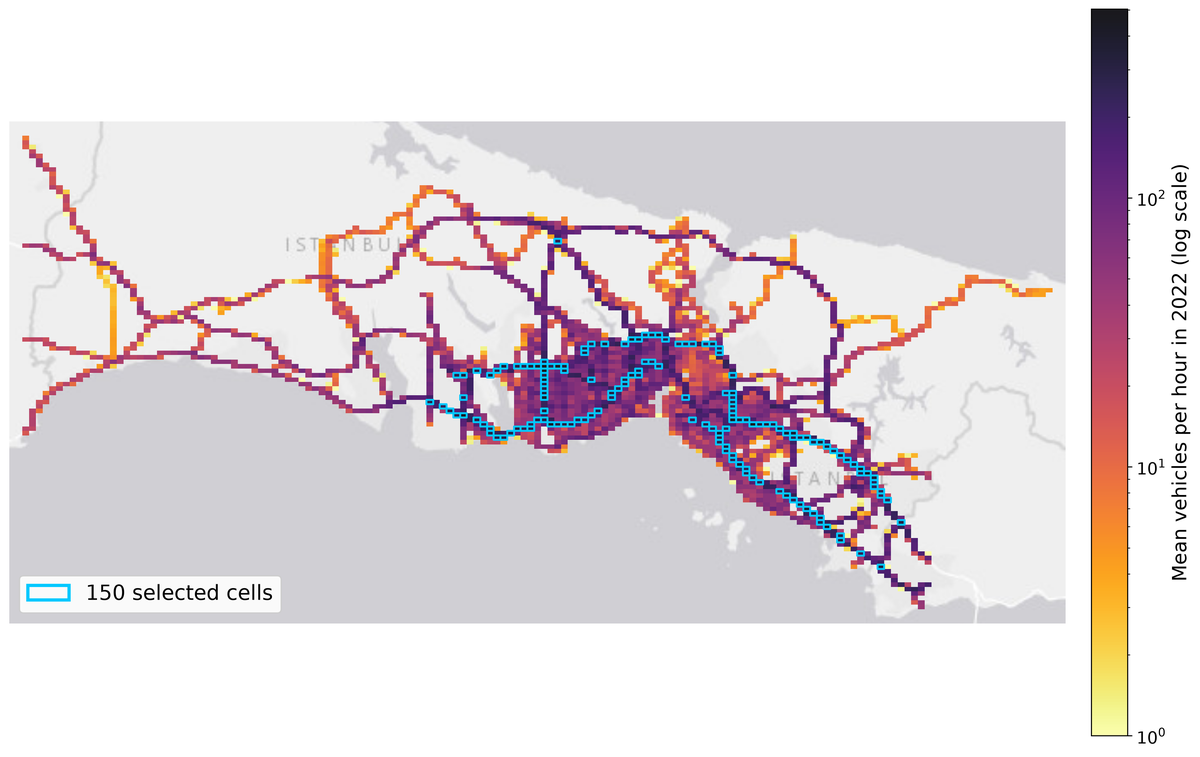
\includegraphics[width=0.82\columnwidth]{fig_map_cells.png}
  \caption{All 2{,}459 cells reporting in 2022, coloured by mean vehicles per hour (log scale); the 150 selected cells are outlined in blue. Base map: Esri, DeLorme, NAVTEQ.}
  \label{fig:map}
\end{figure}


\subsection{Missing hours, outages and calendar}
An hour with no reporting cell is a \emph{city-wide outage} (1{,}544 of 26{,}304 hours); an hour with fewer than half of the usual number of cells is a \emph{partial outage} (53 hours). A \emph{faulty hour} has data but a city mean below 20\% of the median of the same hour of the week in the four weeks before and after (99 hours, including 12 hours on 28 April and the whole of 29 April 2024). Holidays are never flagged. Outage and faulty hours are excluded from scoring by a rule fixed before testing.

A hand-built daily calendar for 2022--2025 adds public holidays, the half-day before a holiday (arife), bridge days, Ramadan, school breaks and special events such as the closures after the earthquake of 6 February 2023. From it we derive a week-after-holiday flag, the days since the last holiday and a target-day group. Between 2022 and 2024 it contains 41 holiday days and 51 days that fall in the week after a holiday.

\subsection{A level break in January 2024}
Around 24 January 2024 the mean weekday count jumps from 271.6 to 491.8 vehicles per cell-hour (60 days before and after, +81.1\%), while the weekend-to-weekday ratio falls from about 0.9 to 0.65 within a week. Real traffic does not change this fast, so we regard it as a change in data collection (an undocumented hypothesis) and also report fold averages without 2024-Q1, a rule fixed in advance.

%% ============================================================
\section{Method}
\subsection{Task and features}
The target is the number of vehicles in a cell in the next hour. All features are computed in DuckDB \cite{raasveldt2019} on the complete hourly grid, where a missing hour becomes an empty row, so that a lag of $k$ rows is exactly $k$ hours and every input comes from the past. The inputs are the current count and speed, the counts 1, 2 and 23 hours back, the count of the same hour one week earlier (168 hours before the target), hour of day (sine and cosine), day of week and a weekend flag of the target hour, the cell position and its mean log count in the training data, and, in the calendar configurations, six flags of the target day.

\subsection{Models, baselines and evaluation}
Four models from standard libraries \cite{pedregosa2011,ke2017} are trained on $\log(1+\text{vehicles})$ and transformed back: Ridge regression \cite{hoerl1970}; Extra Trees with 200 trees \cite{geurts2006}; LightGBM with 600 rounds, learning rate 0.05, 63 leaves and the cell as a categorical feature \cite{ke2017}; and a multilayer perceptron with hidden layers of 64 and 32 units. Settings are fixed, not tuned. Each fit uses 150{,}000 training rows drawn with a fixed random rank; the main configuration is run with three seeds. The baselines are persistence (next hour equals this hour), the same hour last week, the median of the same hour over three weeks, and a historical average.

The year 2022 is used only for training. Each quarter of 2023 and 2024 is in turn the test set, and the model is trained on every hour whose target lies before that quarter, an expanding-window scheme suited to time series \cite{bergmeir2012}. A cell is scored in a quarter only if it reports at least half of its hours; outage and faulty hours are not scored; special-event days are reported separately. We report the mean absolute error (MAE) and the mean absolute scaled error (MASE), the MAE divided by that of persistence in the same quarter \cite{hyndman2006}, as means over the eight quarters with their standard deviation (SD); gaps smaller than the SD are treated as inconclusive.

\subsection{Repair ladder and weekly lag variants}
The repair ladder has six cumulative steps scored on the same cell-hours: R0 raw records with lags taken by row position, as a quick notebook would do; R1 one row per cell and hour (no duplicates were found, so R1 equals R0); R2 the complete hourly grid; R3 outage and faulty hours dropped from training; R4 calendar flags added (the main configuration); R5 a holiday-aware weekly lag.

The five weekly lag variants use only past data: L0 the plain 168-hour lag; L1 no weekly lag; L2 the nearest ordinary week (two weeks back if the previous week was a holiday, three if that was one too); L3 the median of one, two and three weeks back; L4 L0 plus a holiday-last-week flag and the days since the last holiday. L2 is the lag of step R5. Variants are compared with a paired Wilcoxon signed-rank test on daily MAE \cite{wilcoxon1945}.

%% ============================================================
\section{Results}
\subsection{What the data show}
\begin{figure*}[t]
  \centering
  \begin{subfigure}[b]{0.49\textwidth}\centering
    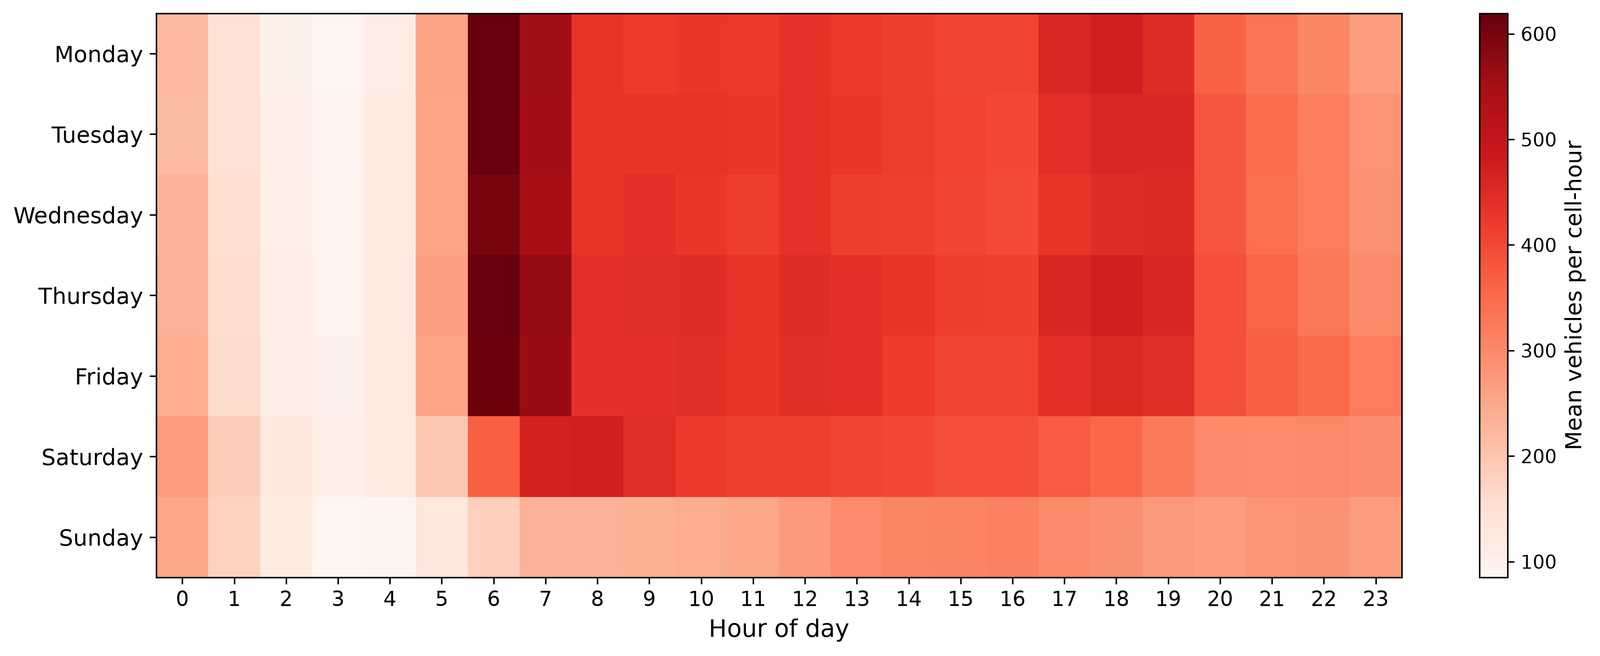
\includegraphics[width=\linewidth]{fig_rq1_heatmap_hour_dow.png}
    \caption{By hour of day and day of week}\label{fig:heat}
  \end{subfigure}\hfill
  \begin{subfigure}[b]{0.49\textwidth}\centering
    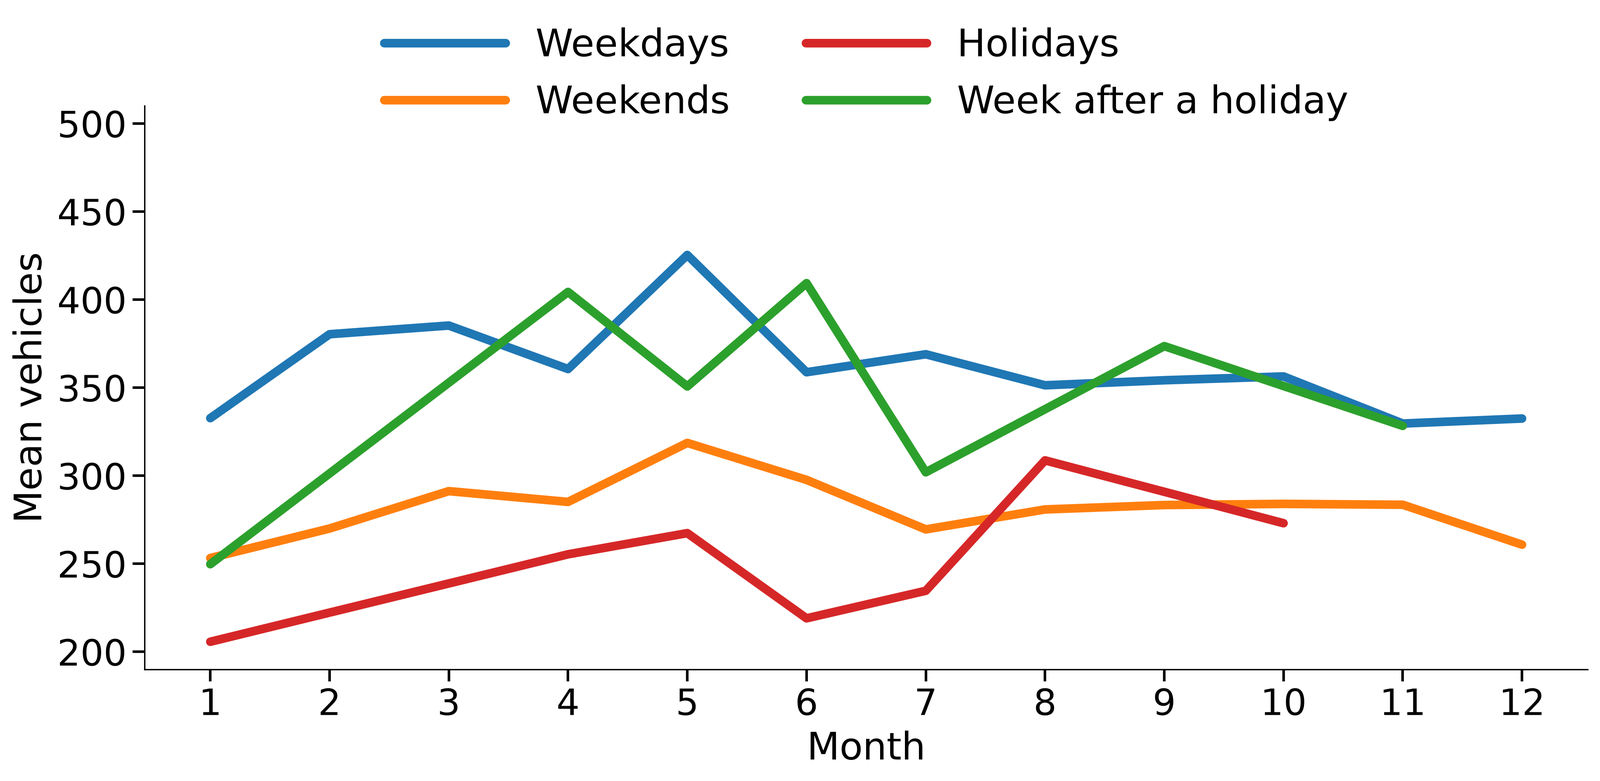
\includegraphics[width=\linewidth]{fig_rq1_hourly_profile.png}
    \caption{By month for four day types}\label{fig:monthly}
  \end{subfigure}
  \caption{Mean vehicles per cell-hour (2022--2024, outage and faulty hours removed). (a) Ordinary days only: a sharp morning peak at 06:00--07:00 on weekdays, flatter weekends. (b) Months without a holiday or a week after a holiday are skipped, so those lines join the nearest months that have one.}
  \label{fig:data}
\end{figure*}

A strong but fragile weekly rhythm. Weekdays share a sharp morning peak at 06:00--07:00 and a lower evening peak, while weekends are flatter (Figure~\ref{fig:heat}). Holidays are the quietest day type in every month that has one (205.7--308.7 vehicles per cell-hour against 329.7--425.4 on weekdays; Figure~\ref{fig:monthly}). The week after a holiday is not a simple return to normal: in April, June and September it is even busier than an ordinary weekday (404.4 against 360.6, 409.4 against 358.8 and 373.6 against 354.2). Relative to weekdays of the same year, holidays are 27.7\% lower in 2022 and 19.5\% lower in 2023; the 2024 value ($-41.2\%$) is inflated by the level break.

The echo is visible before any model is fitted. The count at the same hour one week earlier is, on average, 1.43 times today's count on holidays, 0.76 times in the week after a holiday and 1.00 on ordinary weekdays. A feature that is almost exact on ordinary days is thus biased upwards on holidays and downwards one week later, exactly when the previous week was a holiday.

Gaps come from outages, not from cells. In January 2024 only 54.6\% of cell-hours have a record (338 hours lost city-wide), yet every cell keeps over 50\% coverage in each quarter: gaps hit all cells at once, so row index and clock drift apart.

\subsection{Model comparison}
\begin{table}[t]
  \caption{Next-hour forecast error, mean over eight test quarters (vehicles per cell-hour). SD: standard deviation across quarters; MAE$^{*}$: mean without 2024-Q1, the quarter of the level break.}
  \label{tab:rq2}
  \small
  \setlength{\tabcolsep}{4pt}
  \begin{tabular}{lrrrr}
    \toprule
    Method & MAE & SD & MASE & MAE$^{*}$ \\
    \midrule
    Persistence         & 68.1 & 9.5  & 1.000 & 66.3 \\
    Same hour last week & 60.8 & 20.6 & 0.908 & 63.4 \\
    Median of 3 weeks   & 52.9 & 14.5 & 0.789 & 54.7 \\
    Historical average  & 90.3 & 41.9 & 1.283 & 82.0 \\
    \midrule
    Ridge               & 50.3 & 7.2  & 0.743 & 49.8 \\
    Extra Trees         & 39.9 & 8.7  & 0.588 & 37.4 \\
    LightGBM            & \textbf{37.9} & 6.4 & \textbf{0.563} & \textbf{36.7} \\
    MLP                 & 38.0 & 4.6  & 0.567 & 37.9 \\
    \bottomrule
  \end{tabular}
\end{table}

\begin{figure}[t]
  \centering
  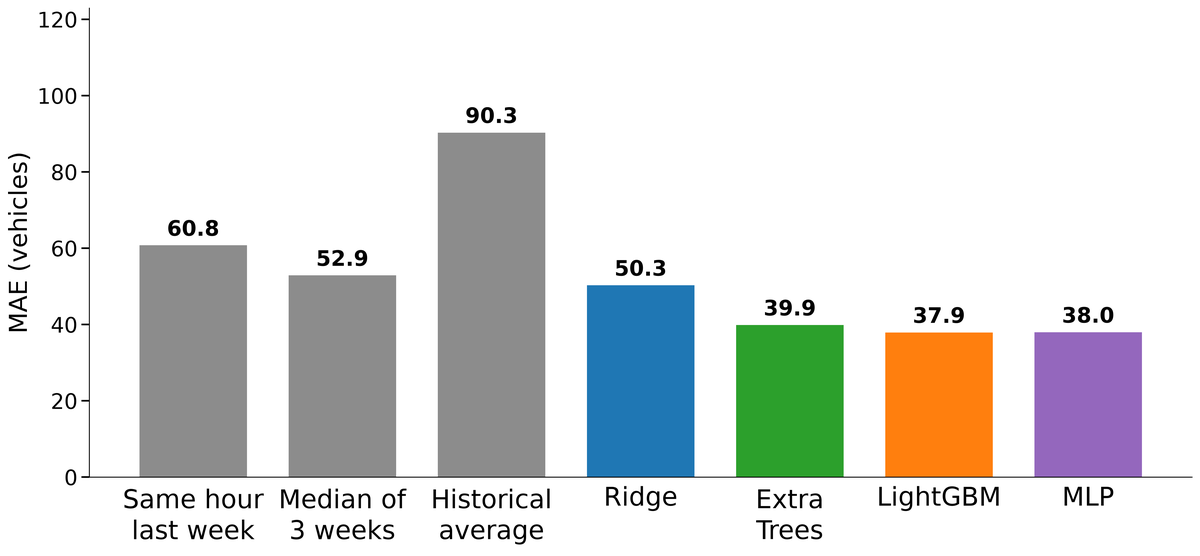
\includegraphics[width=0.85\columnwidth]{fig_rq2_models.png}
  \caption{Mean MAE over eight test quarters for three baselines (grey) and four models. Persistence (68.1) is the MASE reference (Table~\ref{tab:rq2}).}
  \label{fig:models}
\end{figure}

The best three models cannot be separated. LightGBM has the lowest mean MAE (37.9, MASE 0.563), 43.7\% below persistence (Table~\ref{tab:rq2}, Figure~\ref{fig:models}). The MLP (38.0) is practically tied, and the gap to Extra Trees (39.9) is smaller than the quarter-to-quarter SD of any of them (4.6--8.7). Without 2024-Q1 the order changes to LightGBM, Extra Trees, MLP. Only the statement that the three non-linear models beat Ridge (50.3) and all baselines is robust. The spread between seeds is small (0.13 for LightGBM, 0.69 for the MLP) compared with the spread between quarters.

Baselines that copy last week are fragile. The same hour last week (60.8) barely beats persistence and has the largest SD (20.6); the historical average (90.3) is the weakest because it averages hours before the level break.

Where the error sits. Every method has its largest error in the morning rush (06:00--07:00). In the week after a holiday the models' MAE is 46.5--72.8 against 37.3--49.3 on ordinary days, whereas on holidays themselves the models (27.5--39.7) are far better than the weekly baselines (about 132--136), which copy a normal day.

\begin{table}[t]
  \caption{Per test quarter: days in the week after a holiday, MAE of persistence, and MASE of two baselines (SHLW: same hour last week; Med3: median of three weeks) and two models. Values above 1 in bold.}
  \label{tab:quarters}
  \small
  \setlength{\tabcolsep}{3.5pt}
  \begin{tabular}{lrrrrrr}
    \toprule
    Quarter & Days & Pers. & SHLW & Med3 & LGBM & MLP \\
    \midrule
    2023-Q1 & 1  & 59.0 & 0.768 & 0.667 & 0.509 & 0.552 \\
    2023-Q2 & 6  & 58.1 & \textbf{1.169} & 0.985 & 0.643 & 0.689 \\
    2023-Q3 & 7  & 62.8 & \textbf{1.212} & \textbf{1.010} & 0.717 & 0.737 \\
    2023-Q4 & 2  & 58.4 & 0.968 & 0.864 & 0.615 & 0.622 \\
    2024-Q1 & 1  & 80.8 & 0.526 & 0.499 & 0.574 & 0.478 \\
    2024-Q2 & 12 & 75.0 & \textbf{1.352} & \textbf{1.087} & 0.579 & 0.544 \\
    2024-Q3 & 2  & 72.7 & 0.557 & 0.544 & 0.412 & 0.448 \\
    2024-Q4 & 2  & 78.2 & 0.715 & 0.656 & 0.451 & 0.468 \\
    \bottomrule
  \end{tabular}
\end{table}

Quarter by quarter, the echo reappears. Persistence error grows from 58.1--62.8 vehicles in 2023 to 72.7--80.8 in 2024 with the traffic level, yet LightGBM's MASE improves (0.509--0.717 in 2023, 0.412--0.579 in 2024; Table~\ref{tab:quarters}). The weekly baseline is worse than persistence in exactly the three quarters with the most week-after-holiday days (6, 7 and 12 days, against 1--2 elsewhere): a method that copies last week is only as good as last week's calendar.

\subsection{What each repair step is worth}
\begin{table}[t]
  \caption{MAE along the repair ladder on the same test rows (vehicles per cell-hour). $\Delta$: change of the four-model mean from the previous step.}
  \label{tab:ladder}
  \small
  \setlength{\tabcolsep}{3.5pt}
  \begin{tabular}{lrrrrrr}
    \toprule
    Step & Ridge & ET & LGBM & MLP & Mean & $\Delta$ \\
    \midrule
    R0 raw records        & 59.4 & 42.5 & 40.8 & 41.7 & 46.1 & -- \\
    R1 one row per hour   & 59.4 & 42.5 & 40.8 & 41.7 & 46.1 & 0.00 \\
    R2 hourly grid        & 50.7 & 39.9 & 38.1 & 38.9 & 41.9 & \textbf{$-$4.22} \\
    R3 drop outages       & 50.8 & 39.6 & 38.1 & 38.4 & 41.7 & $-$0.16 \\
    R4 calendar           & 50.2 & 39.3 & 37.5 & 37.8 & 41.2 & $-$0.54 \\
    R5 holiday-aware lag  & 48.8 & 38.7 & 37.1 & 38.7 & 40.8 & $-$0.38 \\
    \bottomrule
  \end{tabular}
\end{table}

One step does most of the work. From raw records to the final configuration the mean MAE falls from 46.1 to 40.8 (11.5\%), and 4.22 of these 5.3 vehicles come from R2, the complete hourly grid (Table~\ref{tab:ladder}). On raw records taken in row order, 0.52\% of ``previous hour'' lags and 45.7\% of ``one week earlier'' lags miss the intended time, because one missing hour in the preceding week shifts the rows; Ridge, which uses the lags linearly, gains most (59.4 to 50.7). The later steps ($-0.16$, $-0.54$, $-0.38$) are below the quarter-to-quarter SD, and the MLP even gets worse at R5 (37.8 to 38.7).

Averages hide where the steps act. The grid lowers ordinary-day error from 46.3 to 41.2 and bridge-day error from 54.1 to 41.3, but raises holiday error from 35.1 to 39.6 and week-after error from 50.7 to 54.7. A likely reason is that once the weekly lag points to the right week, it also points to the holiday, and the echo becomes visible; with misaligned rows it was blurred. Calendar flags then lower holiday error from 38.8 to 31.5, and R5 lowers week-after error from 54.2 to 41.8. The steps should therefore be read as a sequence: R2 makes the time axis correct, and only on a correct axis does a holiday-aware lag have something to fix.

\subsection{The holiday echo and the weekly lag}
The echo exists for every model. With the plain lag (L0), the mean MAE of the four models in the week after a holiday is 54.2 against 40.8 on ordinary days, a ratio of 1.33; per model the ratio is 1.24 (MLP), 1.26 (Extra Trees), 1.29 (LightGBM) and 1.47 (Ridge), and 2.1 for the same-hour-last-week baseline. An event study over 16 holiday periods (Table~\ref{tab:event}) locates it: the L0 error is 47.7 in the week before and 38.5 on the first holiday day, then jumps to 66.8 on day $+7$, when the lag looks back at that day, and returns to 47.1 afterwards.

\begin{table}[t]
  \caption{MAE (mean of four models) by days from the first day of a holiday period (day 0), over 16 holiday periods; a window averages the daily values of its days. Best value per column in bold.}
  \label{tab:event}
  \small
  \setlength{\tabcolsep}{3.5pt}
  \begin{tabular}{lrrrrr}
    \toprule
    Variant & $-$7..$-$1 & Day 0 & $+$1..$+$6 & Day $+$7 & $+$8..$+$14 \\
    \midrule
    L0 plain lag      & 47.7 & \textbf{38.5} & 42.2 & 66.8 & 47.1 \\
    L1 no weekly lag  & 50.3 & 46.1 & 44.0 & 67.3 & 47.6 \\
    L2 ordinary week  & 46.0 & 39.3 & 43.2 & 58.5 & 45.7 \\
    L3 median of 3    & \textbf{44.6} & 40.9 & \textbf{39.9} & \textbf{58.3} & \textbf{42.6} \\
    L4 L0 + flags     & 49.1 & 39.2 & 43.7 & 70.3 & 48.4 \\
    \bottomrule
  \end{tabular}
\end{table}

\begin{table}[t]
  \caption{MAE (mean of four models) by target-day group for the five weekly lag variants. Best value per column in bold.}
  \label{tab:lag}
  \small
  \setlength{\tabcolsep}{4pt}
  \begin{tabular}{lrrrr}
    \toprule
    Variant & Ordinary & Holiday & Arife & Week after \\
    \midrule
    L0 plain lag      & 40.8 & 31.5 & \textbf{50.7} & 54.2 \\
    L1 no weekly lag  & 45.5 & \textbf{30.4} & 64.8 & 46.9 \\
    L2 ordinary week  & 41.1 & 32.3 & 52.5 & 41.8 \\
    L3 median of 3    & \textbf{39.5} & 35.8 & 54.9 & \textbf{41.1} \\
    L4 L0 + flags     & 41.6 & 31.8 & 51.0 & 54.6 \\
    \bottomrule
  \end{tabular}
\end{table}

A better lag removes most of it. On day $+7$, L2 and L3 are 8.3 and 8.5 vehicles below L0, whereas the holiday flags of L4 make it worse (3.5 above L0) and removing the lag (L1) costs most on the first holiday day (46.1 against 38.5). Over all week-after-holiday hours, L2 and L3 lower the MAE from 54.2 to 41.8 and 41.1, while on ordinary days L2 costs only 0.2 vehicles and L3 even gains 1.3 (Table~\ref{tab:lag}). Removing the lag is not a fix: it is worse on ordinary days (45.5) and on arife (64.8).

The gain is significant where it is needed. Over the 33 week-after-holiday test days, paired Wilcoxon tests favour L2 and L3 over L0 for all four models (median daily reductions 1.9--9.8 vehicles, $p<0.01$; better on 70--91\% of these days). Over all 630 test days L2 is slightly worse than L0 for LightGBM and the MLP (median $+0.14$ and $+1.02$), a small price for the week-after gain.

Models lean on the weekly lag. Shuffling each feature group \cite{breiman2001,fisher2019} shows that recent traffic dominates (43--58\% of the MAE rise on ordinary days), but the weekly lag takes 33.1\% for Ridge, 17.5\% for the MLP, 13.1\% for LightGBM and 11.1\% for Extra Trees (Table~\ref{tab:impact}). In the week after a holiday these shares drop (26.3, 14.4, 9.3 and 6.8\%): the models learn to distrust the lag only partly, which fits the remaining echo. The shares describe reliance, not causation.

\begin{table}[t]
  \caption{Share (\%) of the summed MAE rise over five feature groups when each group is shuffled (ordinary days); in brackets, the MAE rise in vehicles. ET: Extra Trees; LGBM: LightGBM.}
  \label{tab:impact}
  \small
  \setlength{\tabcolsep}{2.5pt}
  \begin{tabular}{lrrrr}
    \toprule
    Feature group & Ridge & ET & LGBM & MLP \\
    \midrule
    Recent traffic      & \textbf{42.8} (49.7) & \textbf{51.0} (69.1) & \textbf{57.8} (79.8) & \textbf{49.4} (73.5) \\
    Same hour last week & \textbf{33.1} (38.4) & \textbf{11.1} (15.0) & \textbf{13.1} (18.1) & \textbf{17.5} (26.1) \\
    Same hour yesterday & 20.2 (23.4) & 9.7 (13.1)  & 11.1 (15.4) & 15.6 (23.2) \\
    Time of day/week    & 3.3 (3.9)   & 25.1 (34.0) & 15.3 (21.2) & 15.6 (23.2) \\
    All other           & 0.6 (0.7)   & 3.1 (4.3)   & 2.7 (3.7)   & 1.8 (2.7) \\
    \bottomrule
  \end{tabular}
\end{table}

Sensitivity to the training sample. Each fit uses 150{,}000 sampled rows, a limit set by a 16 GB laptop. Refitting Ridge and LightGBM (L0 and L2) on all training rows (1.49 to 2.85 million) in 2023-Q2 and 2024-Q3 changed the all-day MAE by $-0.07$ to $+0.32$ for Ridge and $-0.64$ to $-1.60$ for LightGBM, well below the quarter-to-quarter SD, and L2 stayed below L0 in the week after a holiday in all four cases (by 2.1 to 29.5 vehicles). More data helps LightGBM a little but does not change the conclusions.

%% ============================================================
\section{Discussion and Limitations}
Repair priorities. Three data decisions matter more than choosing among the best models: lags on a true time axis, a holiday-aware weekly lag, and a check for breaks. In practice, check that lags point to the intended time (45.7\% of raw weekly lags did not), report the week after a holiday separately, and track MASE per quarter to spot breaks.

Limitations. The 150 cells are the busiest of 2022, so results may not carry over to quiet roads. The level break is unexplained, and the ranking of the best three models depends on whether 2024-Q1 is included. Holidays are few (16 periods); models use fixed settings, one city and one horizon; the hand-built calendar may miss closures.

Reproducibility. Two notebooks build the data, run the eight folds and write every table and figure of this paper.

%% ============================================================
\section{Conclusion}
On Istanbul open traffic data, boosted trees and a small neural network forecast the next hour about 44\% better than persistence, and the evidence does not separate them. Preparing the data on a complete hourly grid is the single most valuable repair step, worth 4.2 of the 5.3 vehicles gained by all steps. After a holiday the usual weekly lag raises the error of every model by 24 to 47\%, peaking seven days after the holiday starts; the nearest ordinary week or a three-week median removes most of that excess. Open-data forecasting studies should report their time-axis handling, their treatment of holidays and a check for level breaks.

%% ACM authorship policy: any use of generative AI to create content must be disclosed here.
%% Check this sentence against the group's own record of AI use before submission.
\begin{acks}
The authors thank the Istanbul Metropolitan Municipality for publishing the data under an open license. The authors used Claude (Anthropic) to assist with analysis code and language editing; all code, numbers and text were checked by the authors.
\end{acks}

\bibliographystyle{ACM-Reference-Format}
\bibliography{references}

\end{document}
